\section{Software}

\subsection{Overview}

\frame {
 \frametitle{Software Overview}
 \begin{itemize}
  \item Python on the backend
  \begin{enumerate}[A.]
   \item Django for the REST, HTTP stuff
   \item Custom python to interact with Arduino interface
  \end{enumerate}
  \item Heavy Javascript on the frontend
  \begin{enumerate}[A.]
   \item jqplot for creating graphs (jQuery included)
   \item RequireJS for module dependency and loading
   \item BackboneJS for MVC architecture
  \end{enumerate}
 \end{itemize}
}

\frame{
 \frametitle{Backend Overview}
 \begin{itemize}
  \item Django will be used to handle database
  \item Tastypie will be used to prototype the REST API
  \item Django admin will be used to prototype the admin interface
  \item Each functional area of the project will be a Django module
  \begin{enumerate}[A.]
   \item Power Bill Guestimator
   \item Satellite
   \item REST API
  \end{enumerate}
 \end{itemize}
}

\frame{
 \frametitle{Backend Overview}
 \begin{center}
  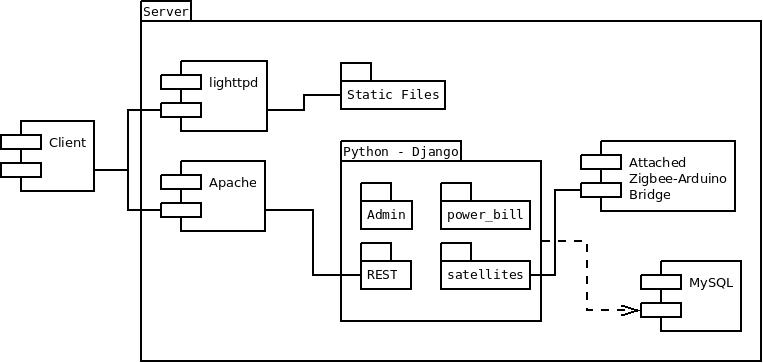
\includegraphics[width=0.8\textwidth]{Diagrams/ServerDependency.jpg}
 \end{center}
}

\frame{
 \frametitle{Frontend Overview}
 \begin{itemize}
  \item RequireJS - Loads all the required modules for each page
  \begin{enumerate}[A.]
   \item Helps keep the scope clean
   \item Enhances modular development
  \end{enumerate}
  \item Backbone.js - MVC Architecture on the client-side
  \item iCanHaz - Provides the 'V' part of MVC
  \item jqplot - Renders charts and graphs
  \item jQuery - Deals with all the behind-the-scenes AJAX stuff
 \end{itemize}
}

\frame{
 \frametitle{Frontend Overview}
 \begin{center}
  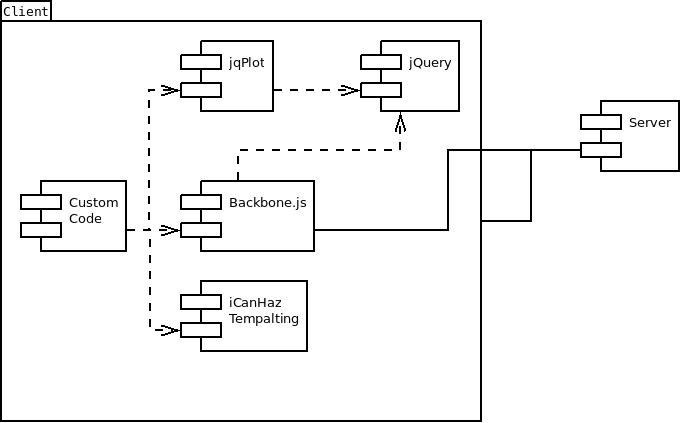
\includegraphics[width=0.8\textwidth]{Diagrams/ClientDependency.jpg}
 \end{center}
}

\subsection{Interesting problems}

\frame{
 \frametitle{Power Bill Guestimator}
 \begin{itemize}
  \item Power companies have different ways of charging
  \begin{enumerate}[A.]
   \item Power consumptions tiers
   \item Prime-time vs Off-time
  \end{enumerate}
  \item Cost of power can fluctuate (over long periods of time)
  \item Need to keep a history
  \item Database-consolidation can't mix power "tiers"
 \end{itemize}
}
 
\frame{
 \frametitle{Power Bill Guestimator Solutions}
 \begin{itemize}
  \item Support all methods of charging power
  \item Store key in data table indicating what power "tier" applies
  \item Calculate current power tier at runtime
  \begin{enumerate}[A.]
   \item Scheduling problem
   \item Calculate during save for efficiency
  \end{enumerate}
 \end{itemize}
}

\frame{
 \frametitle{Limited Resources}
 \begin{itemize}
  \item Server must be low powered
  \begin{enumerate}[A.]
   \item Limited processing power
   \item Limit memory capacity
  \end{enumerate}
  \item Server must store data for years
  \item Server must be able to serve many clients
  \item Server must be online 24/7 with some reliability
  \item Server must be able to process data from all Satellites
 \end{itemize}
}

\frame{
 \frametitle{Limited Resources Solution}
 \begin{itemize}
  \item Bare-bones operating system
  \item Compacting database
  \item Offload templating to clients via Javascript
  \begin{enumerate}[A.]
   \item REST API
   \item JSON
  \end{enumerate}
  \item Use well-known and tested components
  \item Use a database which supports simultaneous read/writes
 \end{itemize}
}

\frame{
 \frametitle{Limited Time}
 \begin{itemize}
  \item We have 2 software engineers, not full time
  \item We have 3 computer engineers, not full time
  \begin{enumerate}[A.]
   \item Most focus on the hardware
  \end{enumerate}
  \item Lots of implied requirements
  \begin{enumerate}[A.]
   \item Access control
   \item Extensible API
   \item History tables
  \end{enumerate}
 \end{itemize}
}

\frame{
 \frametitle{Limited Time - Solutions}
 \begin{itemize}
  \item Modular - Prototype components with the expectation of complete replacements
  \item Open Source - Utilize free libraries
  \item One stone for many birds
  \begin{enumerate}[A.]
   \item Use this project for other classes
   \item Use architecture and design that we're familiar with
   \item Reusable components
  \end{enumerate}
 \end{itemize}
}